\documentclass{article}
\usepackage[polish]{babel}
\usepackage{minted}
\usepackage[letterpaper,top=2cm,bottom=2cm,left=3cm,right=3cm,marginparwidth=1.75cm]{geometry}
\usepackage{amsmath}
\usepackage{graphicx}
\usepackage[colorlinks=true, allcolors=blue]{hyperref}
\usepackage[T1]{fontenc}
\usepackage[table,xcdraw]{xcolor}
\usepackage{float}
\usepackage[figurename=Wykres]{caption}

\title{MOwNiT - Aproksymacja}
\author{Jakub Frączek}

\begin{document}

\maketitle

\section{Funkcja dla której przeprowadzone zostało doświadczenie}

\begin{center}
\(f(x) = 10 * m + \frac{\mathrm{x}_{}^{2}}{k} - 10 * m * cos(k*x)\)
\end{center}

\noindent
gdzie:

\bigbreak

\(k = 1.5\)
\newline \indent
\(m = 3.0\)
\newline \indent
\(x \in [-4\pi, 4\pi]\)

\section{Dane techniczne}

\subsection{Hardware}

Laptop z procesorem Intel Core i5-9300H 2.4GHz oraz 32 GB pamięci RAM.

\subsection{Software}

Wykorzystany został system Windows 11 x64 oraz język Python w wersji 3.11.8 wraz z bibliotekami:
\begin{itemize}
\item math
\item copy
\item matplotlib
\item numpy
\end{itemize}

\section{Aproksymacja}

\noindent
Funkcja bazowe, czyli ciągi jednomianów \(\varphi _j(x) = x^i, j = 0, 1, ..., m\)

\noindent
Funkcja aproksymująca: \(f(x) = \sum_{j=0}^{m}a_j\varphi_j(x) = \sum_{j=0}^{m}a_jx^i00\)

\noindent
F(x) - zadana na zbiorze dyskretnym \(\{x_i\}, i = 0, 1, ..., n\)

\noindent
Szukamy takich współczynników \(a_j\), że:

\[min!\sum_{i=0}^{n}w(x_i)[F(x_i) - f(x_i)]^2\]

\noindent
Układ normalny:

\[\sum_{i = 0}^{n}w(x_i)[F(x_i) - \sum_{j=0}^{m}a_jx_i^j]x_i^{k\longleftarrow \frac{\partial f}{\partial a_k}} = 0, k = 0, 1, ..., m\]

\[\sum_{i = 0}^{n}w(x_i)x_i^k\sum_{j=0}^{m}a_jx_i^j = \sum_{i=0}^{n}w(x_i)F(x_i)x_i^k, k =0,1,...,m\]

\[\sum_{j=0}^{m}(\sum_{i=0}^{n}w(x_i)x_i^{j+k}a_j = \sum_{i=0}^{n}w(x_i)F(x_i)x_i^k\]

\noindent
W postaci macierzowej:

\begin{gather*}
\begin{pmatrix}
\Sigma w_i & \Sigma w_ix_i & \Sigma w_ix_i^2 & \cdots & \Sigma w_ix_i^m \\
\Sigma w_ix_i & \Sigma w_ix_i^2 & \Sigma w_ix_i^3 & \cdots & \Sigma w_ix_i^{m+1} \\
\vdots & \vdots & \vdots & \ddots & \vdots \\
\Sigma w_ix_i^m & \Sigma w_ix_i^{m+1} & \Sigma w_ix_i^{m+2} & \cdots & \Sigma w_ix_i^{2m} 
\end{pmatrix} 
\begin{pmatrix}
a_0 \\
a_1 \\
\vdots \\
a_m 
\end{pmatrix}
= 
\begin{pmatrix}
\Sigma w_iF_i \\
\Sigma w_iF_ix_i \\
\vdots \\
\Sigma w_iF_ix_i^m 
\end{pmatrix}
\end{gather*}

\[G \cdot A=B\]

\section{Metody szacowania błędu przybliżenia funkcji}

Wszystkie błędy zostały policzone z dokładnością do 100 równoodległych punktów.

\subsection{Największa różnica wartości funkcji}

Największa różnica między wartością funkcji aproksymowanej, a funkcji aproksymującej:

\begin{center}
    \(\max_{x\in [a, b]} |F(x) - \mathrm{P}_{n}^{}(x)|\)
\end{center}

\subsection{Błąd średniokwadratowy}

Suma kwadratów różnic mięcy wartością funkcji aproksymowanej, a funkcji aproksymującej podzielona przez liczba punktów, w których wykonujemy porównanie:

\begin{center}
\(\frac{1}{N} * \sum_{i = 1}^{N}\mathrm{(F(\mathrm{x}_{i}^{}) - \mathrm{P}_{n}^{}(\mathrm{x}_{i}^{}))}_{}^{2}\)
\end{center}

\section{Analiza}

Podczas analizy funkcji aproksymującej,
węzły oraz stopnie wielomianów dobrałem zgodnie z poniższym twierdzeniem:

\begin{center}
Jeżeli \(x_1, x_2, ...,x_n\) są różne oraz m \(\le \) n, to G \(\neq \) 0
\end{center}

\newpage

\section{Przebieg funkcji dla wybranej liczby węzłów}
\subsection{Dla 10 węzłów}

Jak widać na poniższych wykresach (wykres 1, wykres 2, wykres 3, wykres 4) przybliżenie to nie jest za dobre. Najlepszą aproksymację otrzymałem dla 10 stopnia wielomianu. Widać także, że błąd średniokwadratowy wychodzi dość mały przez to, że funkcja aproksymująca przechodzi mniej wiecej przez "środek" funkcji aproksymowanej.

\begin{figure}[H]
  \begin{minipage}[b]{0.49\textwidth}
    \begin{minipage}[b]{\textwidth}
      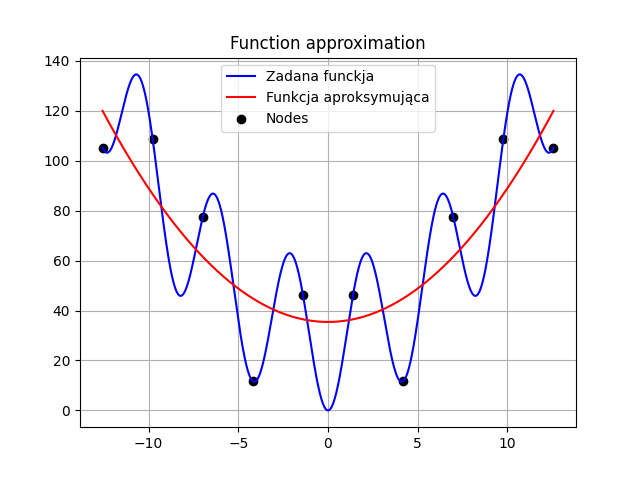
\includegraphics[width=\textwidth]{img02.png}
      \caption{Wielomian 3 stopnia}
    \end{minipage}
    \vspace*{\fill}
    \begin{minipage}[b]{\textwidth}
      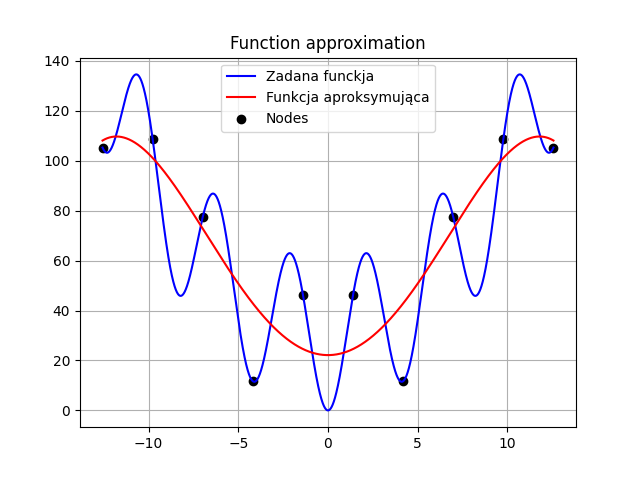
\includegraphics[width=\textwidth]{img03.png}
      \caption{Wielomian 5 stopnia}
    \end{minipage}
  \end{minipage}
  \hfill
  \begin{minipage}[b]{0.49\textwidth}
    \begin{minipage}[b]{\textwidth}
      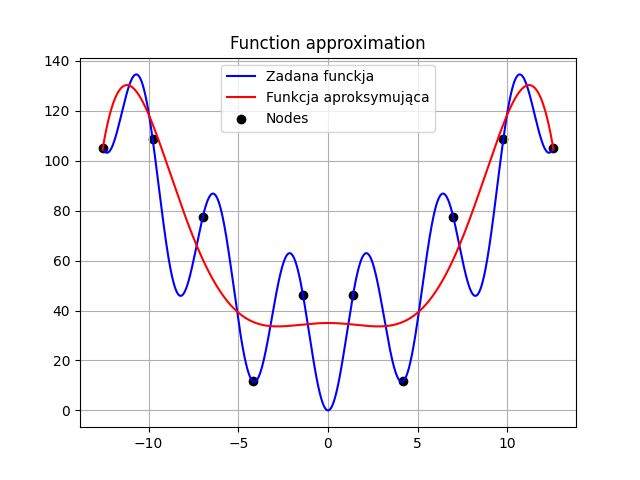
\includegraphics[width=\textwidth]{img04.png}
      \caption{Wielomian 8 stopnia}
    \end{minipage}
    \vspace*{\fill}
    \begin{minipage}[b]{\textwidth}
      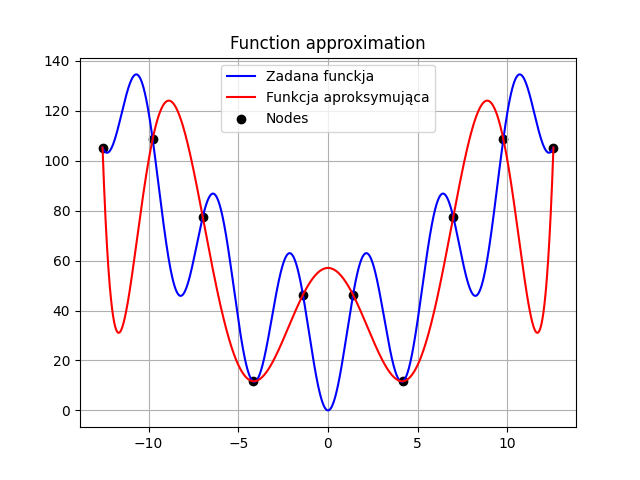
\includegraphics[width=\textwidth]{img05.png}
      \caption{Wielomian 10 stopnia}
    \end{minipage}
  \end{minipage}
\end{figure}

Poniżej, na wykresie 5 przedstawione zostały wartości błędów dla wszystkich możliwych stopni wielomianu.

\begin{figure}[H]
  \centering
  \begin{minipage}[b]{0.4\textwidth}
    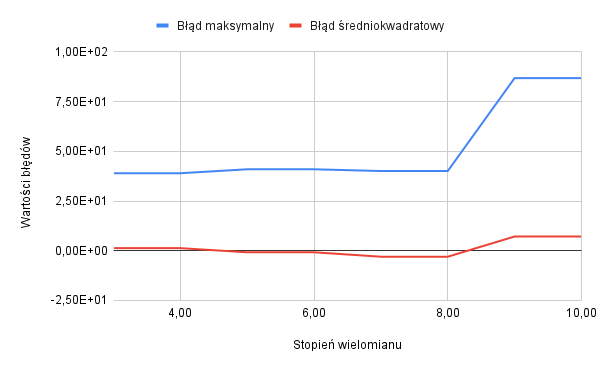
\includegraphics[width=\textwidth]{img14.png}
    \caption{Wartości błędów}
  \end{minipage}
\end{figure}

\newpage

\subsection{Dla 20 węzłów}

W tym przypadku wartości błędów nadal nie są najlepsze, najlepsze przybliżenia otrzymałem dla wielomianu 14 stopnia. Jak widać na poniższych 4 wykresach (wykres 6, wykres 7, wykres 8, wykres 9) dokładność przybliżenia rośnie wraz z wzrostem stopni wielomianu, jednak już przy stopniu zbliżonym do ilości węzłów uwidacznia się efekt Rungego.

\begin{figure}[H]
  \begin{minipage}[b]{0.49\textwidth}
    \begin{minipage}[b]{\textwidth}
      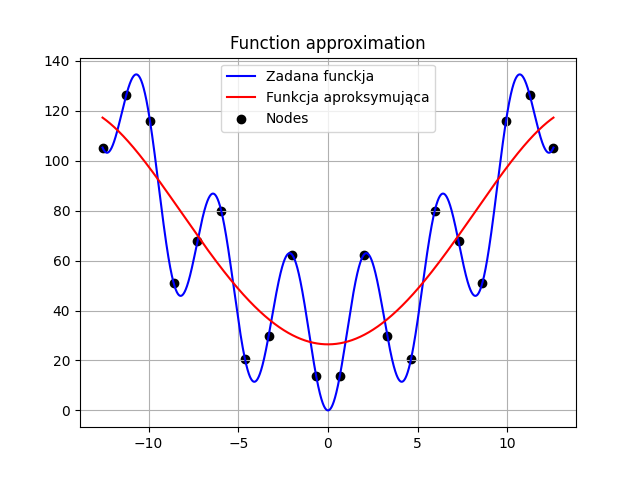
\includegraphics[width=\textwidth]{img06.png}
      \caption{Wielomian 5 stopnia}
    \end{minipage}
    \vspace*{\fill}
    \begin{minipage}[b]{\textwidth}
      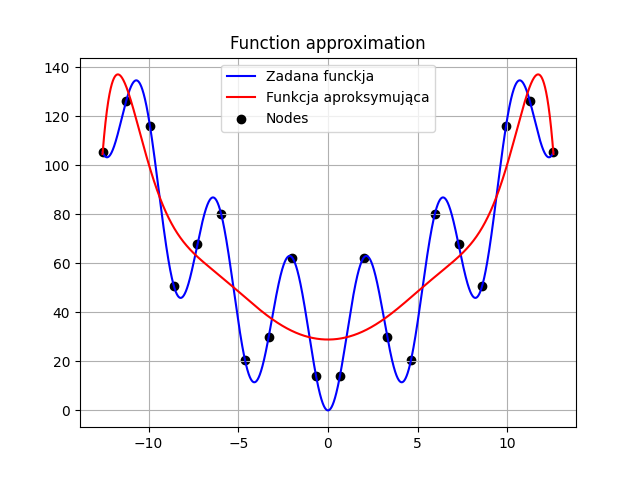
\includegraphics[width=\textwidth]{img07.png}
      \caption{Wielomian 12 stopnia}
    \end{minipage}
  \end{minipage}
  \hfill
  \begin{minipage}[b]{0.49\textwidth}
    \begin{minipage}[b]{\textwidth}
      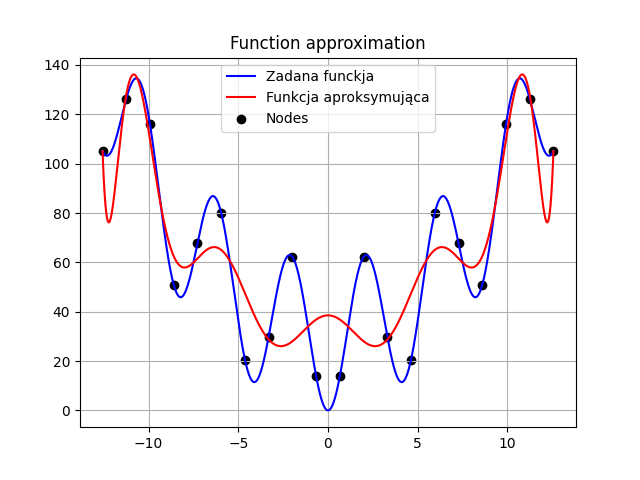
\includegraphics[width=\textwidth]{img08.png}
      \caption{Wielomian 14 stopnia}
    \end{minipage}
    \vspace*{\fill}
    \begin{minipage}[b]{\textwidth}
      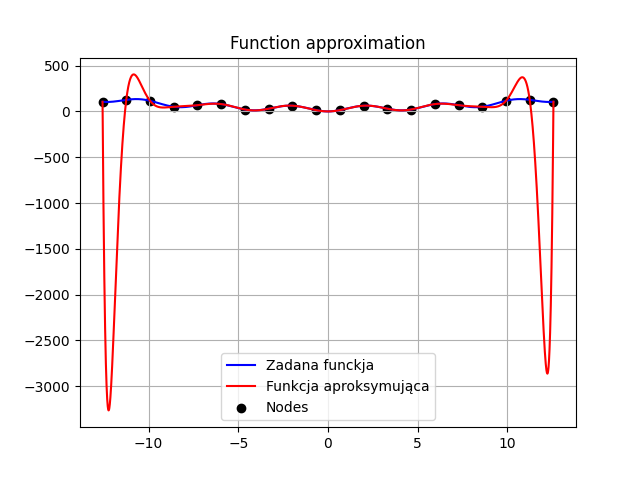
\includegraphics[width=\textwidth]{img09.png}
      \caption{Wielomian 20 stopnia}
    \end{minipage}
  \end{minipage}
\end{figure}

Poniżej, na wykresie 10 przedstawione zostały wartości błędów dla wszystkich możliwych stopni wielomianu.

\begin{figure}[H]
  \centering
  \begin{minipage}[b]{0.4\textwidth}
    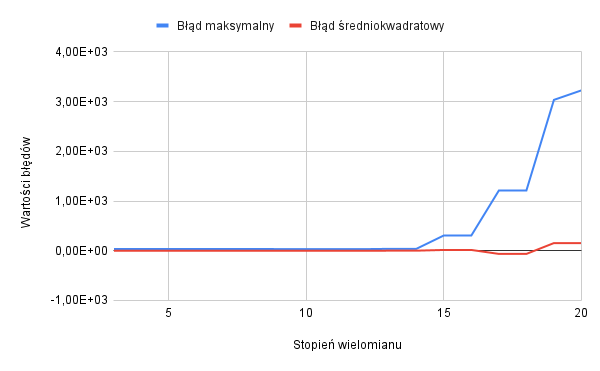
\includegraphics[width=\textwidth]{img15.png}
    \caption{Wartości błędów}
  \end{minipage}
\end{figure}

\newpage

\subsection{Dla 30 węzłów}

Dla 30 węzłów już można otrzymać dośc lepiej dopasowaną funkcję, jednak od 17 stopnia w górę bardzo szybko uwidacznia się efekt Rungego (wykres 11, wykres 12, wykres 13, wykres 14).

\begin{figure}[H]
  \begin{minipage}[b]{0.49\textwidth}
    \begin{minipage}[b]{\textwidth}
      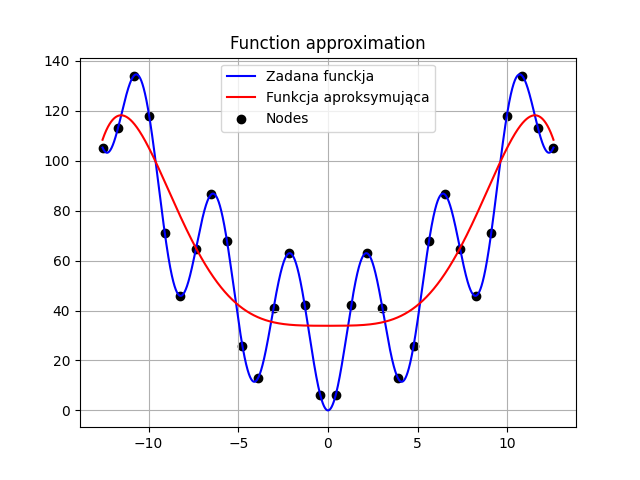
\includegraphics[width=\textwidth]{img10.png}
      \caption{Wielomian 7 stopnia}
    \end{minipage}
    \vspace*{\fill}
    \begin{minipage}[b]{\textwidth}
      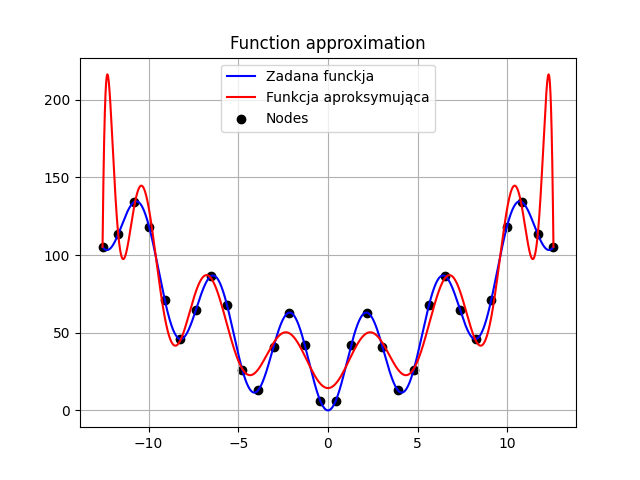
\includegraphics[width=\textwidth]{img11.png}
      \caption{Wielomian 17 stopnia}
    \end{minipage}
  \end{minipage}
  \hfill
  \begin{minipage}[b]{0.49\textwidth}
    \begin{minipage}[b]{\textwidth}
      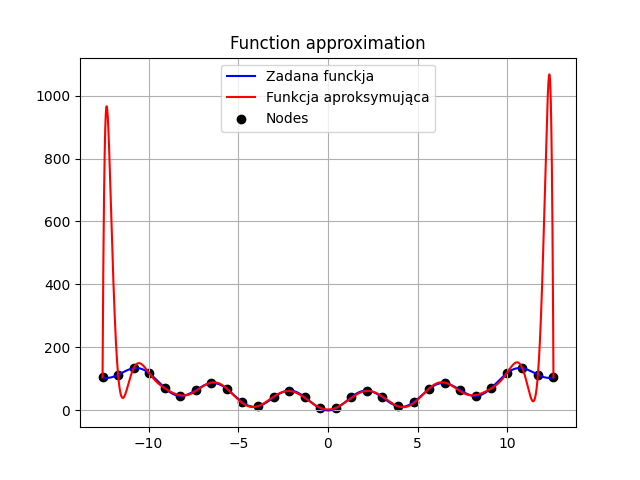
\includegraphics[width=\textwidth]{img12.png}
      \caption{Wielomian 23 stopnia}
    \end{minipage}
    \vspace*{\fill}
    \begin{minipage}[b]{\textwidth}
      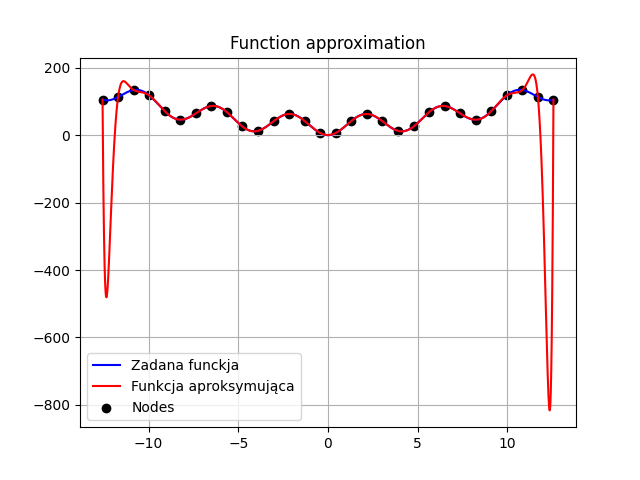
\includegraphics[width=\textwidth]{img13.png}
      \caption{Wielomian 30 stopnia}
    \end{minipage}
  \end{minipage}
\end{figure}

Poniżej, na wykresie 15 przedstawione zostały wartości błędów dla wszystkich możliwych stopni wielomianu.

\begin{figure}[H]
  \centering
  \begin{minipage}[b]{0.4\textwidth}
    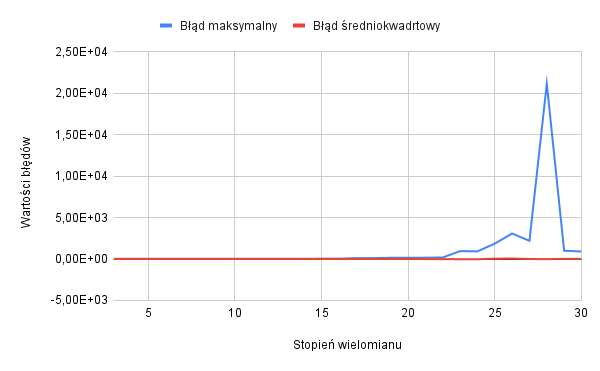
\includegraphics[width=\textwidth]{img16.png}
    \caption{Wartości błędów}
  \end{minipage}
\end{figure}

\newpage

\subsection{Dla 50 węzłów}

Dla 50 węzłów przybliżenie jest juz naprawdę dokładne, oczywiście poza krańcami przedziału, w których wraz ze wzrostem stopnia wielomianu wzrasta błąd przybliżenia, co zostało pokazane na poniższych wykresach (wykres 16, wykres 17, wykres 18 i wykres 19).

\begin{figure}[H]
  \begin{minipage}[b]{0.49\textwidth}
    \begin{minipage}[b]{\textwidth}
      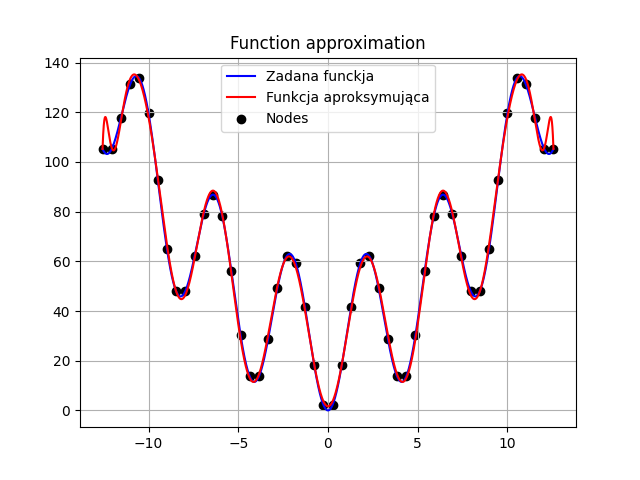
\includegraphics[width=\textwidth]{img18.png}
      \caption{Wielomian 21 stopnia}
    \end{minipage}
    \vspace*{\fill}
    \begin{minipage}[b]{\textwidth}
      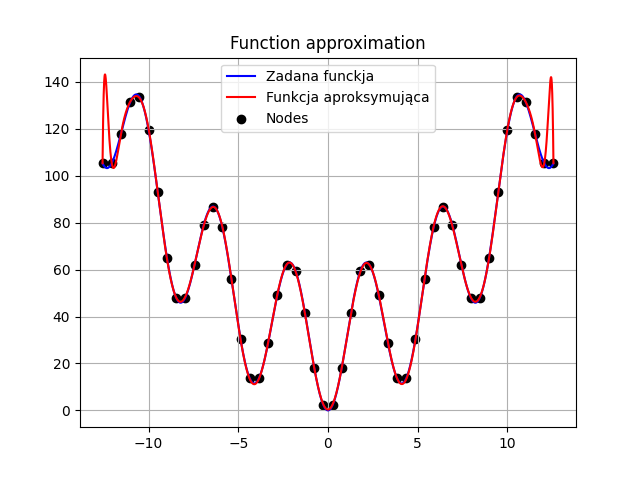
\includegraphics[width=\textwidth]{img19.png}
      \caption{Wielomian 33 stopnia}
    \end{minipage}
  \end{minipage}
  \hfill
  \begin{minipage}[b]{0.49\textwidth}
    \begin{minipage}[b]{\textwidth}
      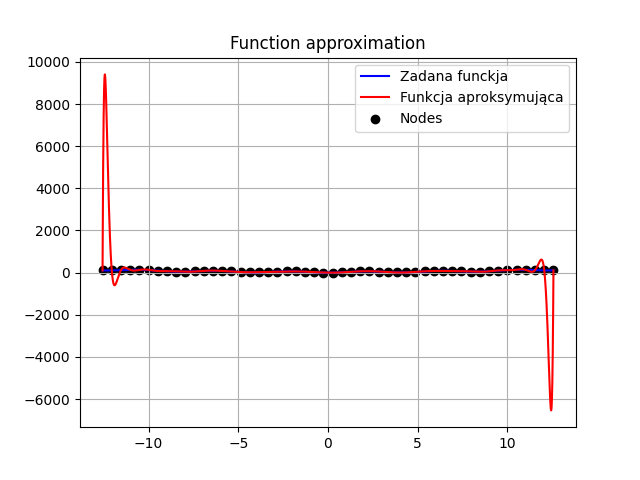
\includegraphics[width=\textwidth]{img20.png}
      \caption{Wielomian 41 stopnia}
    \end{minipage}
    \vspace*{\fill}
    \begin{minipage}[b]{\textwidth}
      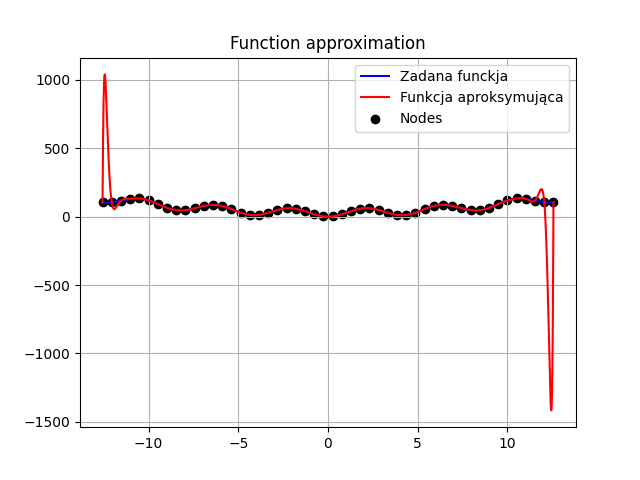
\includegraphics[width=\textwidth]{img21.png}
      \caption{Wielomian 50 stopnia}
    \end{minipage}
  \end{minipage}
\end{figure}

Poniżej, na wykresie 20 przedstawione zostały wartości błędów dla wszystkich możliwych stopni wielomianu.

\begin{figure}[H]
  \centering
  \begin{minipage}[b]{0.4\textwidth}
    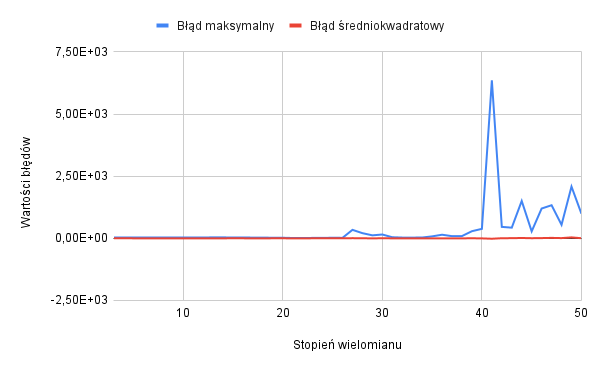
\includegraphics[width=\textwidth]{img22.png}
    \caption{Wartości błędów}
  \end{minipage}
\end{figure}

\newpage

\subsection{Dla 100 węzłów}

W tym przypadku przybliżenie jest najdokładniejsze dla 23 stopnia wielomianiu, a następnie delikatnie oscyluje i w końcu znacznie się pogarsza (wykres 21, wykres 22, wykres 23 i wykres 24).

\begin{figure}[H]
  \begin{minipage}[b]{0.49\textwidth}
    \begin{minipage}[b]{\textwidth}
      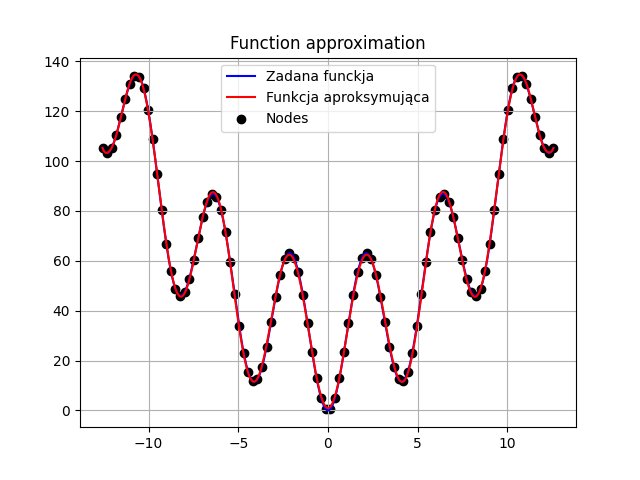
\includegraphics[width=\textwidth]{img23.png}
      \caption{Wielomian 23 stopnia}
    \end{minipage}
    \vspace*{\fill}
    \begin{minipage}[b]{\textwidth}
      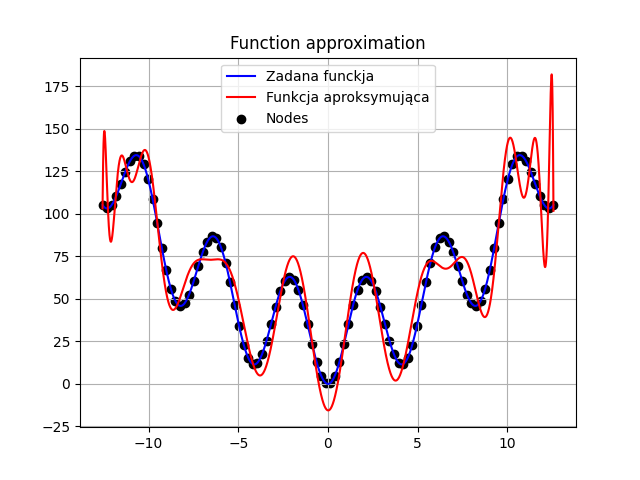
\includegraphics[width=\textwidth]{img24.png}
      \caption{Wielomian 28 stopnia}
    \end{minipage}
  \end{minipage}
  \hfill
  \begin{minipage}[b]{0.49\textwidth}
    \begin{minipage}[b]{\textwidth}
      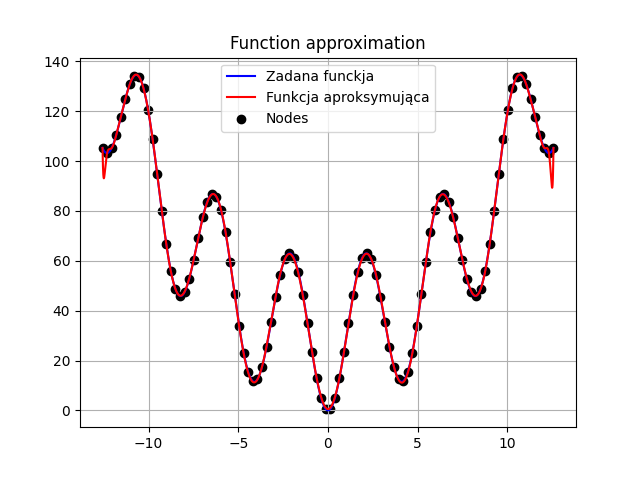
\includegraphics[width=\textwidth]{img25.png}
      \caption{Wielomian 60 stopnia}
    \end{minipage}
    \vspace*{\fill}
    \begin{minipage}[b]{\textwidth}
      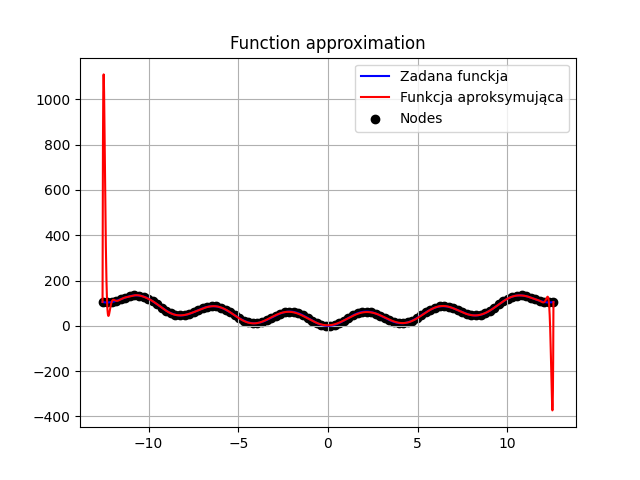
\includegraphics[width=\textwidth]{img26.png}
      \caption{Wielomian 100 stopnia}
    \end{minipage}
  \end{minipage}
\end{figure}

Poniżej, na wykresie 25 przedstawione zostały wartości błędów dla wszystkich możliwych stopni wielomianu.

\begin{figure}[H]
  \centering
  \begin{minipage}[b]{0.4\textwidth}
    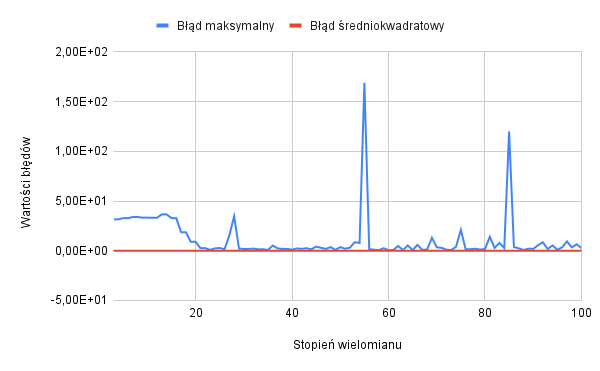
\includegraphics[width=\textwidth]{img27.png}
    \caption{Wartości błędów}
  \end{minipage}
\end{figure}

\newpage

\section{Przebieg funkcji dla wybranego stopnia wielomianu}

jak widać na poniższych wykresach (wykres 26, wykres 27, wykres 28, wykres 29) dla 10 stopnia wielomianu nie otrzymamy dobrego przybliżenia.

\subsection{Dla 10 stopnia}

\begin{figure}[H]
  \begin{minipage}[b]{0.49\textwidth}
    \begin{minipage}[b]{\textwidth}
      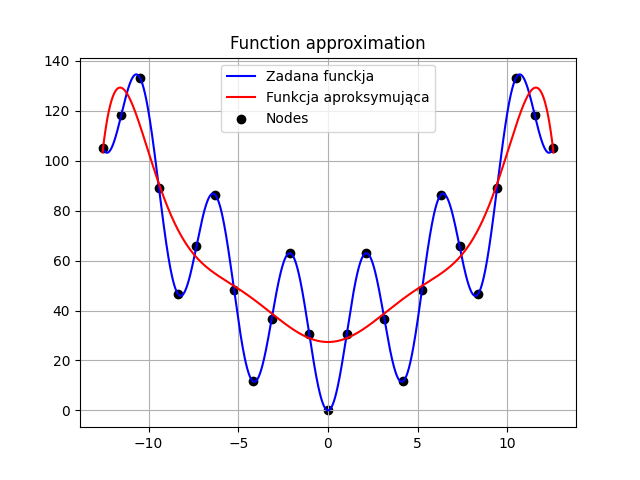
\includegraphics[width=\textwidth]{img28.png}
      \caption{Dla 25 węzłów}
    \end{minipage}
    \vspace*{\fill}
    \begin{minipage}[b]{\textwidth}
      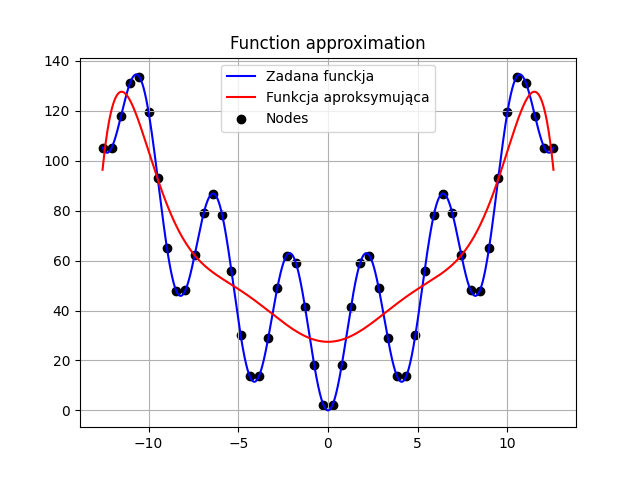
\includegraphics[width=\textwidth]{img29.png}
      \caption{Dla 50 węzłów}
    \end{minipage}
  \end{minipage}
  \hfill
  \begin{minipage}[b]{0.49\textwidth}
    \begin{minipage}[b]{\textwidth}
      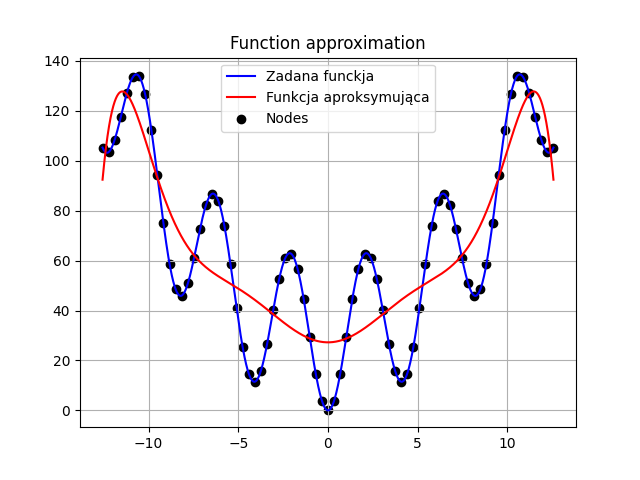
\includegraphics[width=\textwidth]{img30.png}
      \caption{Dla 75 węzłów}
    \end{minipage}
    \vspace*{\fill}
    \begin{minipage}[b]{\textwidth}
      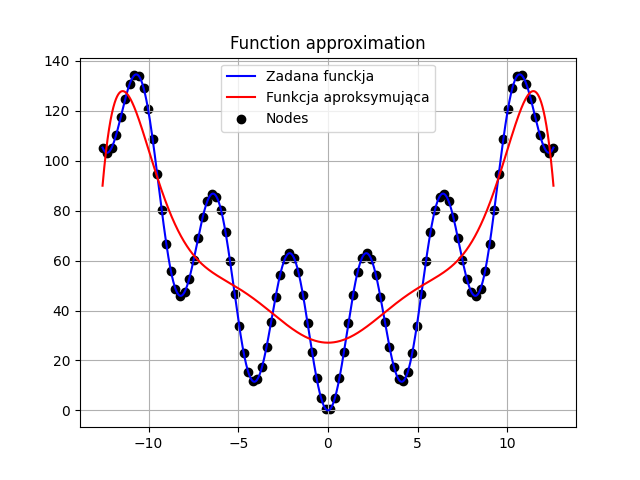
\includegraphics[width=\textwidth]{img31.png}
      \caption{Dla 100 węzłów}
    \end{minipage}
  \end{minipage}
\end{figure}

Poniżej, na wykresie 30 przedstawione zostały wartości błędów dla wszystkich możliwych stopni wielomianu.

\begin{figure}[H]
  \centering
  \begin{minipage}[b]{0.4\textwidth}
    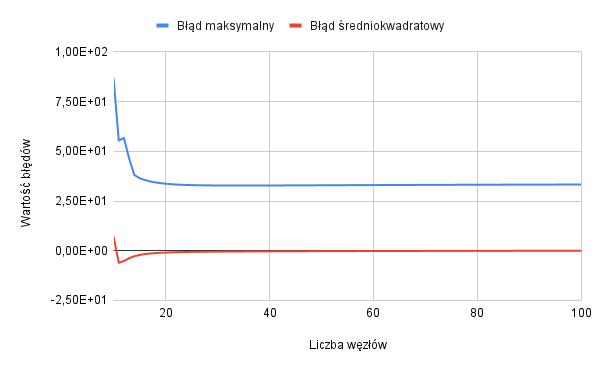
\includegraphics[width=\textwidth]{img32.png}
    \caption{Wartości błędów}
  \end{minipage}
\end{figure}

\subsection{Dla 20 stopnia}

Sytuacja dla 20 stopnia jest dużo lepsza od poprzedniej, gdzyż tutaj dla odpowiedznio dużej liczby węzłów można otrzymać dość zadowalające przybliżenie. Można zauważyć (wykres 31, wykres 32, wykres 33, wykres 34), że wraz ze wzrostem liczby węzłów maleje niedokładnosć na krańcach przedziałów. W tym przypadku najlepsze przybliżenie otrzymałem dla 75 węzłów

\begin{figure}[H]
  \begin{minipage}[b]{0.49\textwidth}
    \begin{minipage}[b]{\textwidth}
      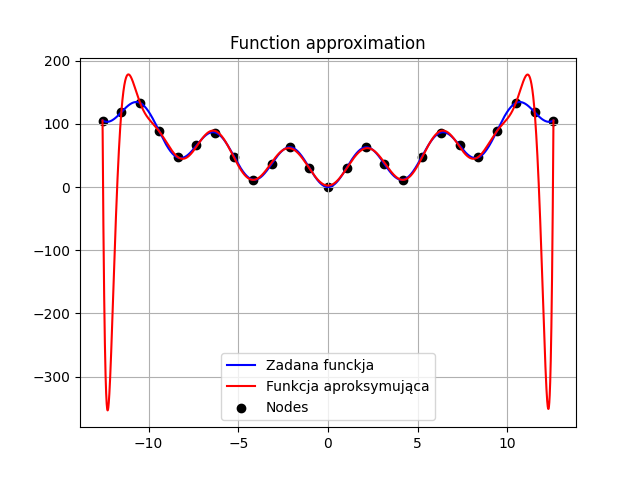
\includegraphics[width=\textwidth]{img33.png}
      \caption{Dla 25 węzłów}
    \end{minipage}
    \vspace*{\fill}
    \begin{minipage}[b]{\textwidth}
      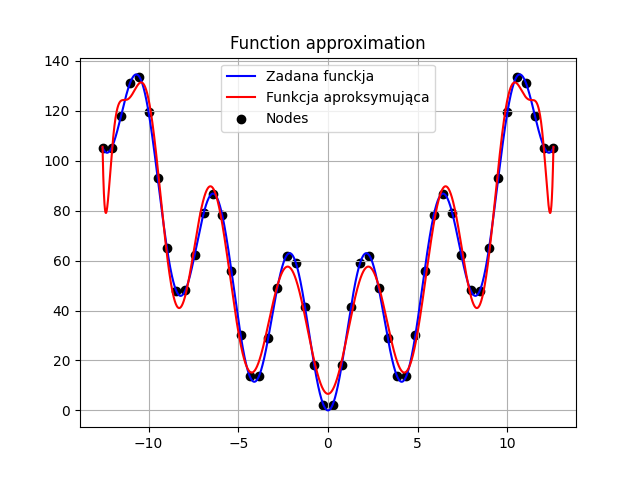
\includegraphics[width=\textwidth]{img34.png}
      \caption{Dla 50 węzłów}
    \end{minipage}
  \end{minipage}
  \hfill
  \begin{minipage}[b]{0.49\textwidth}
    \begin{minipage}[b]{\textwidth}
      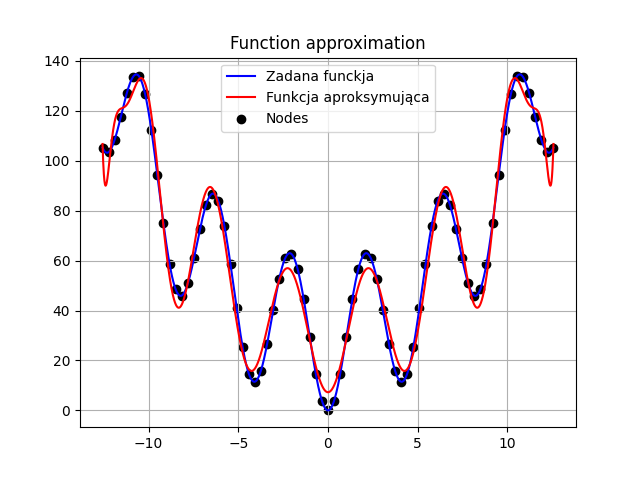
\includegraphics[width=\textwidth]{img35.png}
      \caption{Dla 75 węzłów}
    \end{minipage}
    \vspace*{\fill}
    \begin{minipage}[b]{\textwidth}
      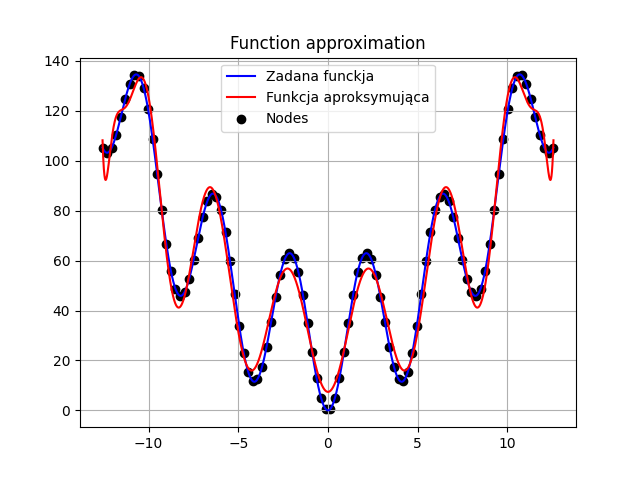
\includegraphics[width=\textwidth]{img36.png}
      \caption{Dla 100 węzłów}
    \end{minipage}
  \end{minipage}
\end{figure}

Poniżej, na wykresie 35 przedstawione zostały wartości błędów dla wszystkich możliwych stopni wielomianu.

\begin{figure}[H]
  \centering
  \begin{minipage}[b]{0.4\textwidth}
    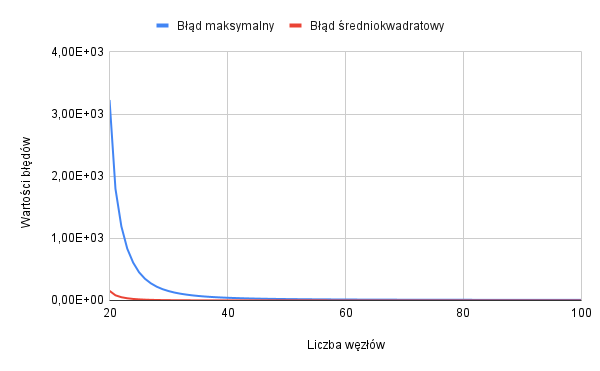
\includegraphics[width=\textwidth]{img37.png}
    \caption{Wartości błędów}
  \end{minipage}
\end{figure}

\newpage

\subsection{Dla 30 stopnia}

Dla wielomianu 30-go stopnia najlepsze przybliżenie otrzymałem dla 52 węzłów (wykres 37). Później wraz ze wzrostem węzłów dochodziło do znacznej oscylacji dokładności przybliżenia i na wykresach 38 i 39 pokazane są teże dość dokładne przybliżenia dla większej ilości węzłów. Natomiast dla 32 węzłów (wykres 36) widać znaczy błąd przybliżenia.

\begin{figure}[H]
  \begin{minipage}[b]{0.49\textwidth}
    \begin{minipage}[b]{\textwidth}
      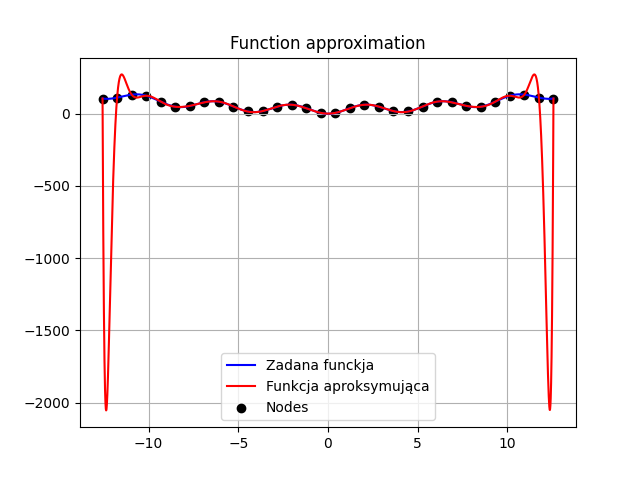
\includegraphics[width=\textwidth]{img38.png}
      \caption{Dla 32 węzłów}
    \end{minipage}
    \vspace*{\fill}
    \begin{minipage}[b]{\textwidth}
      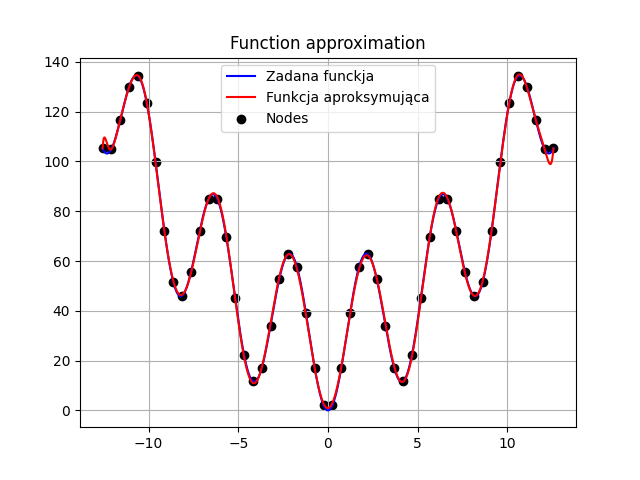
\includegraphics[width=\textwidth]{img39.png}
      \caption{Dla 52 węzłów}
    \end{minipage}
  \end{minipage}
  \hfill
  \begin{minipage}[b]{0.49\textwidth}
    \begin{minipage}[b]{\textwidth}
      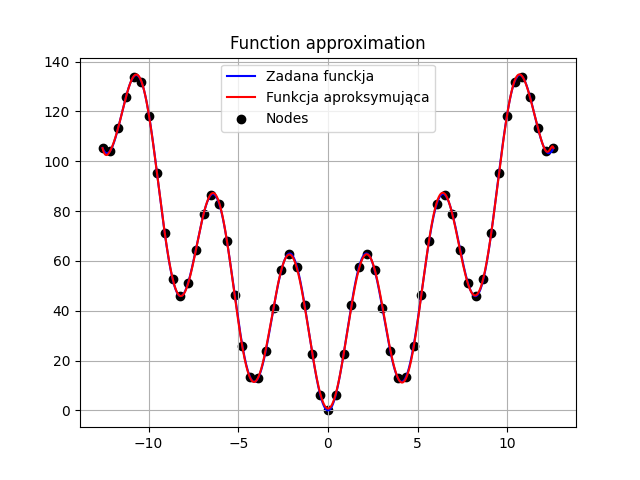
\includegraphics[width=\textwidth]{img40.png}
      \caption{Dla 59 węzłów}
    \end{minipage}
    \vspace*{\fill}
    \begin{minipage}[b]{\textwidth}
      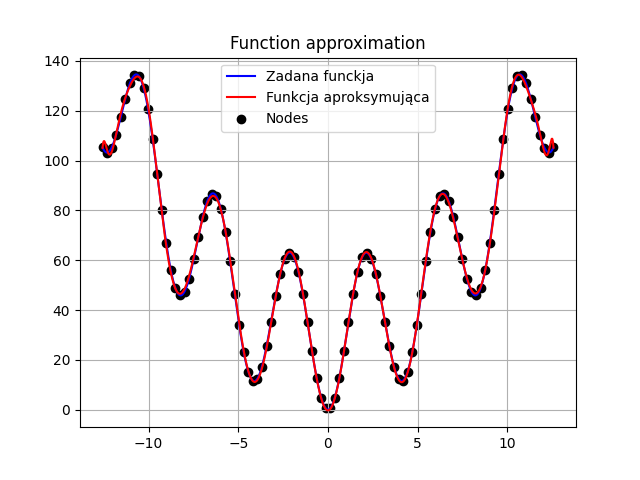
\includegraphics[width=\textwidth]{img41.png}
      \caption{Dla 100 węzłówa}
    \end{minipage}
  \end{minipage}
\end{figure}

Poniżej, na wykresie 40 przedstawione zostały wartości błędów dla wszystkich możliwych stopni wielomianu.

\begin{figure}[H]
  \centering
  \begin{minipage}[b]{0.4\textwidth}
    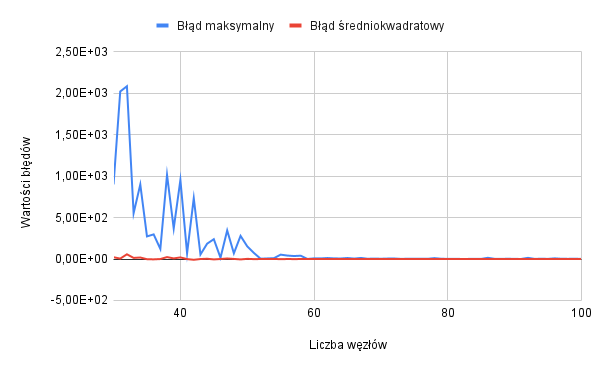
\includegraphics[width=\textwidth]{img42.png}
    \caption{Wartości błędów}
  \end{minipage}
\end{figure}

\subsection{Dla 50 stopnia}

Ja widać na poniższych wykresach (wykres 41, wykres 42, wykres 43, wykres 44) aproksymacje są już dużo gorsze niż w przypadku wielomianiu 30-go stopnia i pogarszają się wraz z wzrostem liczby węzłów.

\begin{figure}[H]
  \begin{minipage}[b]{0.49\textwidth}
    \begin{minipage}[b]{\textwidth}
      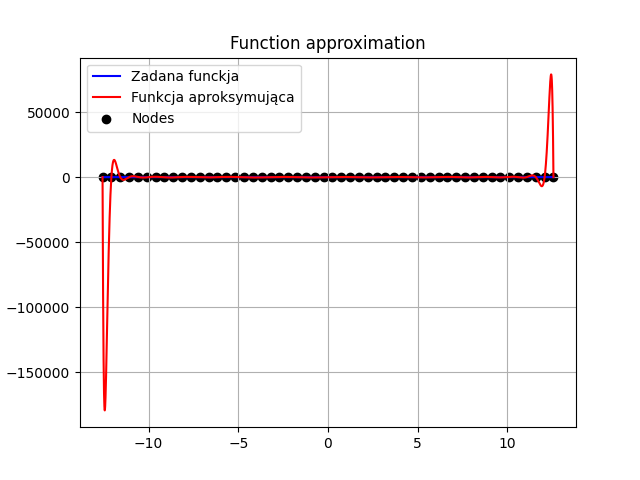
\includegraphics[width=\textwidth]{img43.png}
      \caption{Dla 52 węzłów}
    \end{minipage}
    \vspace*{\fill}
    \begin{minipage}[b]{\textwidth}
      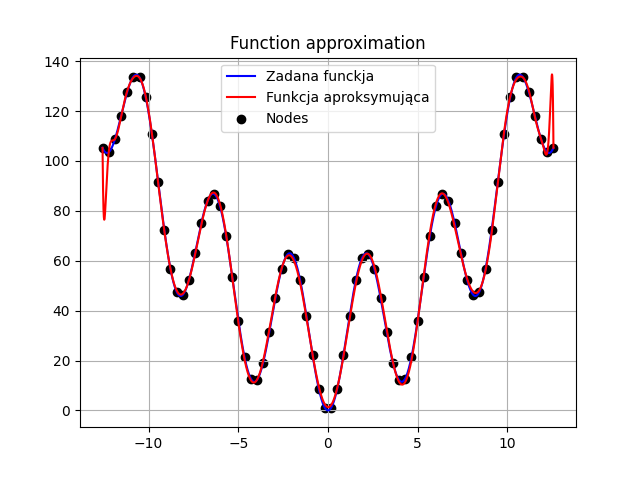
\includegraphics[width=\textwidth]{img44.png}
      \caption{Dla 74 węzłów}
    \end{minipage}
  \end{minipage}
  \hfill
  \begin{minipage}[b]{0.49\textwidth}
    \begin{minipage}[b]{\textwidth}
      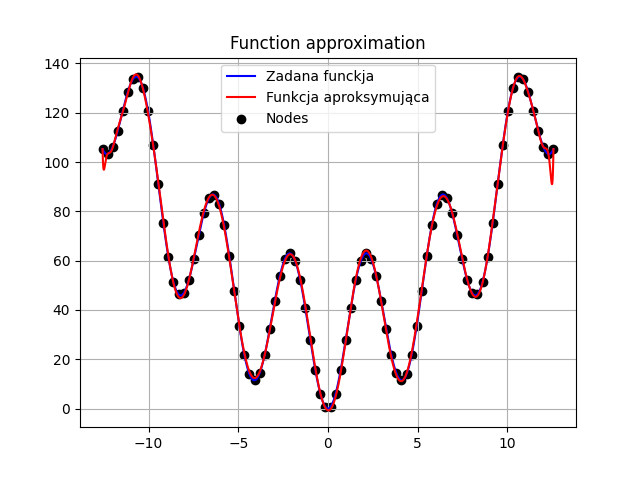
\includegraphics[width=\textwidth]{img45.png}
      \caption{Dla 90 węzłów}
    \end{minipage}
    \vspace*{\fill}
    \begin{minipage}[b]{\textwidth}
      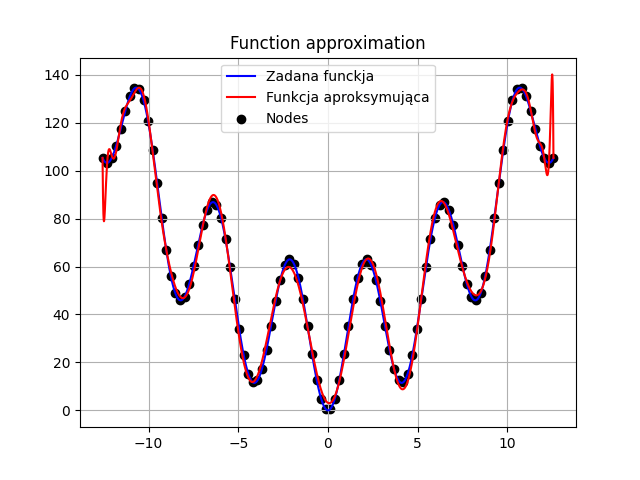
\includegraphics[width=\textwidth]{img46.png}
      \caption{Dla 100 węzłówa}
    \end{minipage}
  \end{minipage}
\end{figure}

Poniżej, na wykresie 45 przedstawione zostały wartości błędów dla wszystkich możliwych stopni wielomianu.

\begin{figure}[H]
  \centering
  \begin{minipage}[b]{0.4\textwidth}
    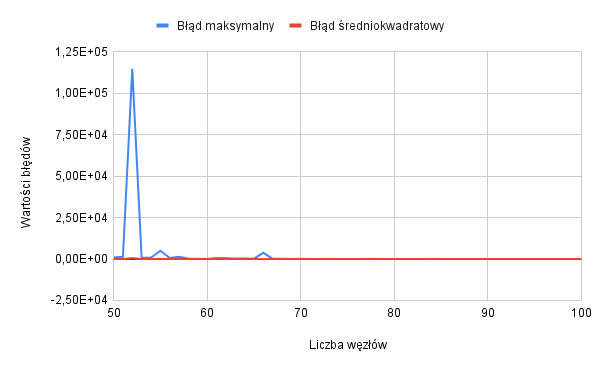
\includegraphics[width=\textwidth]{img47.png}
    \caption{Wartości błędów}
  \end{minipage}
\end{figure}

\newpage

\section{Efekt Rungego}

Na podstawie poprzednich podpunktów można z pewnością stwierdzić, że efekt Rungego występował bardzo często podczas aproksymacji wielomianowej. Najbardziej widoczny był dla 40 węzłów i wielomianu 37-go stopnia. Ta sytuacja została pokazana na wykresie poniżej, a błąd tego przybliżenia w tabelce pod wykresem.

\begin{figure}[H]
  \centering
  \begin{minipage}[b]{0.4\textwidth}
    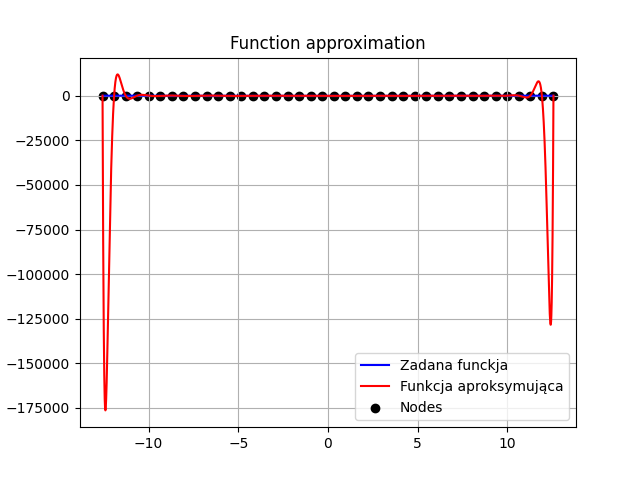
\includegraphics[width=\textwidth]{img49.png}
    \caption{Najlepsze przybliżenie funkcji}
  \end{minipage}
\end{figure}

\begin{table}[!ht]
    \centering
    \begin{tabular}{|l|l|}
    \hline
        Błąd maksymalny & 176413.32885002135    \\ \hline
        Błąd średniokwadratowy & 3832.7665755629732 \\ \hline
        
    \end{tabular}
\end{table}

\section{Najlepsze przyblizenie funkcji}

Najlepsze przybliżenie aproksymowanej funkcji otrzymałem dla 94 węzłów i wielomianu 26 stopnia, został on pokazany na poniższym wykresie, a jego błąd maksymalny i średniokwadratowy poniżej w tabelce. Można powiedzieć, że jest to naprawdę dobre przybliżenie.

\begin{figure}[H]
  \centering
  \begin{minipage}[b]{0.4\textwidth}
    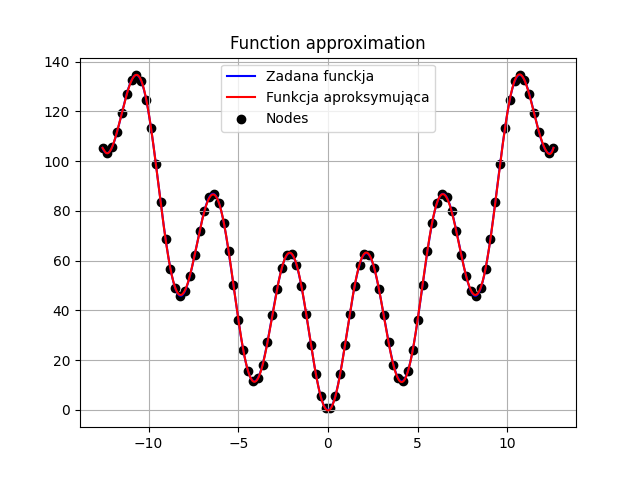
\includegraphics[width=\textwidth]{img48.png}
    \caption{Najlepsze przybliżenie funkcji}
  \end{minipage}
\end{figure}

\begin{table}[!ht]
    \centering
    \begin{tabular}{|l|l|}
    \hline
        Błąd maksymalny & 0.5014720569615605   \\ \hline
        Błąd średniokwadratowy & 0.0017181768299556364 \\ \hline
        
    \end{tabular}
\end{table}

\newpage

\section{Wnioski}

\begin{itemize}
\item Zwiększanie stopnia wielomianu dla ustalonej liczby węzłów powoduje zwiększejnie dokładności przybliżenia tylko do pewnego stopnia, potem zaczyna się zwiększać efekt Rungego i przybliżenie jest coraz gorsze
\item Zwiększanie liczby węzłów dla ustalonego stopnia wielomianu prowadzi do zwiększenia dokładności przyblizenia.
\item Wielomiany o dużym stopniu (30, 40, 50, ...) bardzo często stają się coraz mniej dokładne
\end{itemize}

\end{document}
